%!TEX root = main.tex
\chapter{Introduction to MCMC}\label{ch:mcmc}

Once the problems get to a sufficient complexity, the analytical tools and approximations we have employed in previous chapters will no longer work well.  In those cases, we turn to simulation techniques, one of which is Markov Chain Monte Carlo (MCMC).  It is well beyond this book to talk about the details of this process, but the basic process is the following.

We start with a model of the system, such as the bent coin model in Section~\ref{sec:continuous}.  In that system, we try to estimate the probability that a particular doing will flip heads, quantified by the parameter $\theta$ which can take on values from $\theta=0$ (i.e. a coin which only flips tails) through $\theta=0.5$ (i.e. a ``fair'' coin which flips tails and heads equally) up to $\theta=1$ (i.e. a coin which only flips heads).  Our data consists of a total number of flips, $N$, and how many are heads, $h$.  Although this problem can be done analytically, it is instructive to walk through the solved problem with the new method before looking at more complex models.

MCMC proceeds, roughly, with the following steps

\be
\i Many random ``walkers'' are constructed, each with a random value of the parameters (e.g. $\theta$ in this case).  
\i The random values are chosen from the {\em prior} probability of the parameters.  (e.g. uniform in this case, $P(\theta)=1$)
\i The ``walkers'' move around randomly, guided by the likelihood function (e.g. the Binomial or Bernoulli distribution, in this case)
\i Over hundreds or thousands of steps, the distribution of the values being explored by the ``walkers'' matches the {\em posterior} distribution, so one can look at histograms of the resulting ``walkers'' to get estimates of the parameters, and their uncertainty
\ee

\section{One-Dimensional Models}

The model we first look at is the coin flip model: given 17 heads in 25 flips, what is the probability distribution of the the measure of the coin's bent-ness, $\theta$.  We know the solution is of the form of a beta distribution, but we perform the same analysis with the MCMC technique.  

\begin{Shaded}
\begin{Highlighting}[]
\NormalTok{h,N=data=}\DecValTok{17}\NormalTok{,}\DecValTok{25}
\end{Highlighting}
\end{Shaded}

\begin{Shaded}
\begin{Highlighting}[]
\KeywordTok{def} \NormalTok{P_data(data,theta):}
    \NormalTok{h,N=data}
    \NormalTok{distribution=Bernoulli(h,N)}
    \KeywordTok{return} \NormalTok{distribution(theta)}
\end{Highlighting}
\end{Shaded}

\begin{Shaded}
\begin{Highlighting}[]
\NormalTok{model=MCMCModel(data,P_data,}
                \NormalTok{theta=Uniform(}\DecValTok{0}\NormalTok{,}\DecValTok{1}\NormalTok{))}
\end{Highlighting}
\end{Shaded}

\begin{marginfigure}
\centering
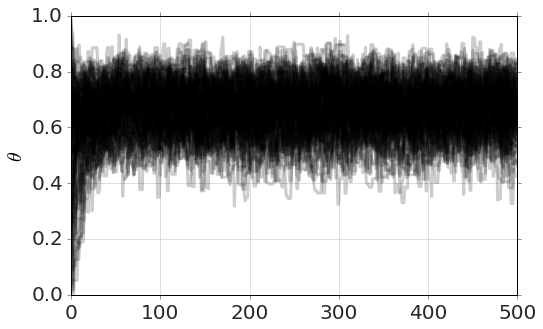
\includegraphics{SIE_MCMC/output_6_2.png}
\caption{So-called MCMC ``chains'' for parameter $\theta$ versus time.  Observe that the values of  $\theta$  start spread evenly from 0 to 1 at the beginning and then thin down to a range of about 0.5-0.8 with the middle around 0.7 (17/25 = 0.68).}
\end{marginfigure}

\begin{Shaded}
\begin{Highlighting}[]
\NormalTok{model.run_mcmc(}\DecValTok{500}\NormalTok{)}
\NormalTok{model.plot_chains()}
\end{Highlighting}
\end{Shaded}

\subsection{Reading the Output}

We can now plot the distributions of the parameters, just $\theta$ in this case, yielding best-fits, uncertainties, etc...



\begin{Shaded}
\begin{Highlighting}[]
\NormalTok{model.plot_distributions()}
\end{Highlighting}
\end{Shaded}

(see Figure~\ref{fig:theta_dist})
\begin{figure*}
\centering
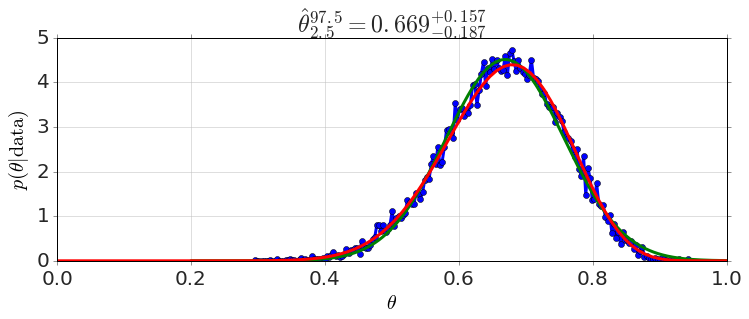
\includegraphics{SIE_MCMC/output_10_1.png}
\caption{Distribution of $\theta$, and the 95\% credible interval.}
\label{fig:theta_dist}
\end{figure*}

We can further perform some simple calculations on the probabilities for the parameters, such as

\begin{Shaded}
\begin{Highlighting}[]
\NormalTok{model.P(}\StringTok{'theta>0.5'}\NormalTok{)}
\end{Highlighting}
\end{Shaded}

\begin{verbatim}
0.96173333333333333
\end{verbatim}

\begin{Shaded}
\begin{Highlighting}[]
\NormalTok{model.P(}\StringTok{'(0.2<theta) & (theta<.5)'}\NormalTok{)}
\end{Highlighting}
\end{Shaded}

\begin{verbatim}
0.038266666666666664
\end{verbatim}


\section{Multi-Dimensional Models}

It is straightforward then to include more than one parameter and to do regression using this technique.  For example, here is an example with some artificial data,


\begin{Shaded}
\begin{Highlighting}[]
\KeywordTok{def} \NormalTok{linear(x,a,b):}
    \KeywordTok{return} \NormalTok{a*x+b}

\NormalTok{model=MCMCModel_Regression(x,y,linear,}
                \NormalTok{a=Uniform(-}\DecValTok{10}\NormalTok{,}\DecValTok{10}\NormalTok{),}
                \NormalTok{b=Uniform(}\DecValTok{0}\NormalTok{,}\DecValTok{100}\NormalTok{),}
                \NormalTok{)}
\end{Highlighting}
\end{Shaded}
\begin{marginfigure}
\centering
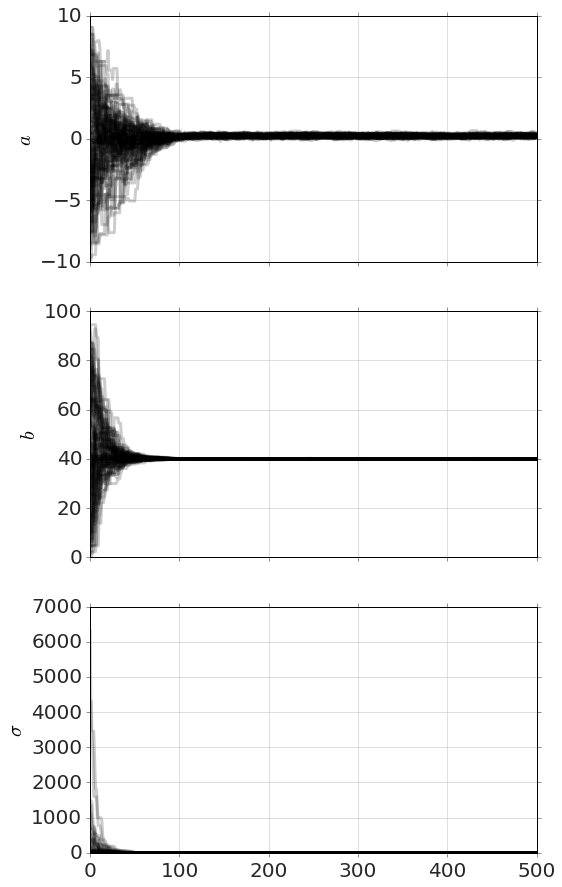
\includegraphics{SIE_MCMC/output_21_2.png}
\caption{Chains for parameters $a$, $b$, and the noise $\sigma$.}
\end{marginfigure}
\begin{Shaded}
\begin{Highlighting}[]
\NormalTok{model.run_mcmc(}\DecValTok{500}\NormalTok{)}
\NormalTok{model.plot_chains()}
\end{Highlighting}
\end{Shaded}


\begin{Shaded}
\begin{Highlighting}[]
\NormalTok{plot(x,y,}\StringTok{'o'}\NormalTok{)}
\NormalTok{model.plot_predictions(xfit,color=}\StringTok{'g'}\NormalTok{)}
\end{Highlighting}
\end{Shaded}

\begin{figure}[htbp]
\centering
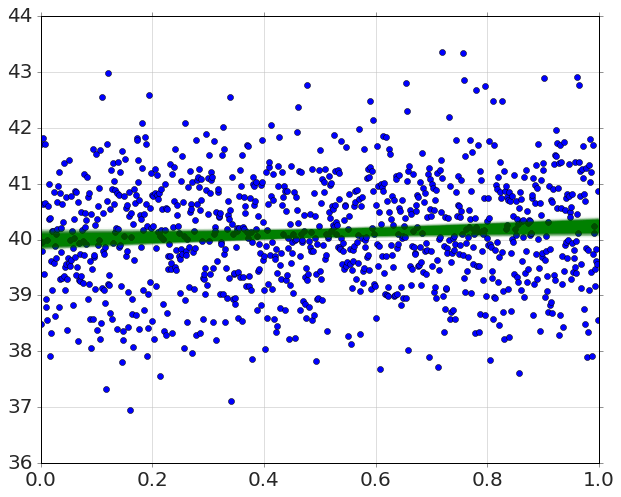
\includegraphics{SIE_MCMC/output_22_0.png}
\caption{Data (blue) and predictions (green) for the model - the width of the predictions demonstrates the uncertainty.}
\end{figure}

\begin{Shaded}
\begin{Highlighting}[]
\NormalTok{model.plot_distributions()}
\end{Highlighting}
\end{Shaded}

\begin{figure}[htbp]
\centering
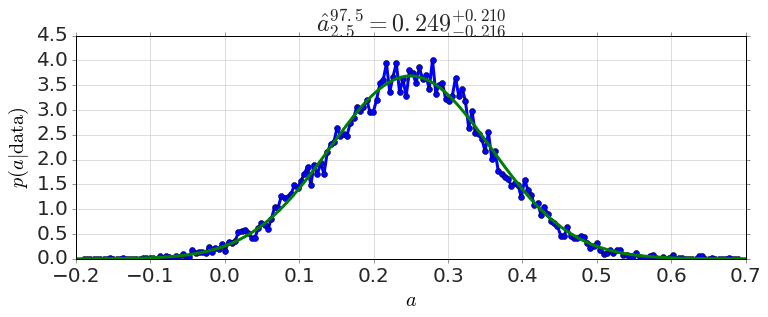
\includegraphics{SIE_MCMC/output_23_0.png}
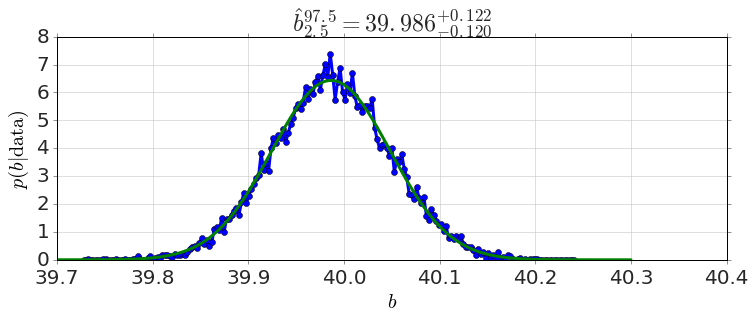
\includegraphics{SIE_MCMC/output_23_1.png}
\caption{Distributions for parameters $a$ and $b$ (slope and intercept).}
\end{figure}

And we can look at best estimates, quartiles, and probability comparisons,

\begin{Shaded}
\begin{Highlighting}[]
\NormalTok{model.percentiles([}\DecValTok{5}\NormalTok{,}\DecValTok{50}\NormalTok{,}\DecValTok{95}\NormalTok{])}
\end{Highlighting}
\end{Shaded}

\begin{verbatim}
{'_sigma': array([ 0.97143798,  1.00744104,  1.0467333 ]),
 'a': array([ 0.07063144,  0.24939562,  0.42523751]),
 'b': array([ 39.88446461,  39.98633744,  40.09010139])}
\end{verbatim}

\begin{Shaded}
\begin{Highlighting}[]
\NormalTok{model.P(}\StringTok{'a>0'}\NormalTok{)}
\end{Highlighting}
\end{Shaded}

\begin{verbatim}
0.98936000000000002
\end{verbatim}




\section{Hierarchical Model Example - Kruschke BEST Test}

A comparison between means is a standard statistical technique.  However, using a {\em hierarchical} model can be superior to the typical tests.\cite{kruschke2013bayesian}

In this example, we use the Kruschke \emph{BEST} Test to compare the difference between a treatment and control - we want to obtain the best estimate of the difference between the means of variables.  With the MCMC technique, we can achieve it with the following,

\begin{Shaded}
\begin{Highlighting}[]
\CharTok{from} \NormalTok{sie }\CharTok{import} \NormalTok{*}
\end{Highlighting}
\end{Shaded}

\begin{Shaded}
\begin{Highlighting}[]
\NormalTok{drug = (}\DecValTok{101}\NormalTok{,}\DecValTok{100}\NormalTok{,}\DecValTok{102}\NormalTok{,}\DecValTok{104}\NormalTok{,}\DecValTok{102}\NormalTok{,}\DecValTok{97}\NormalTok{,}\DecValTok{105}\NormalTok{,}\DecValTok{105}\NormalTok{,}\DecValTok{98}\NormalTok{,}
        \DecValTok{101}\NormalTok{,}\DecValTok{100}\NormalTok{,}\DecValTok{123}\NormalTok{,}\DecValTok{105}\NormalTok{,}\DecValTok{103}\NormalTok{,}\DecValTok{100}\NormalTok{,}\DecValTok{95}\NormalTok{,}\DecValTok{102}\NormalTok{,}\DecValTok{106}\NormalTok{,}
        \DecValTok{109}\NormalTok{,}\DecValTok{102}\NormalTok{,}\DecValTok{82}\NormalTok{,}\DecValTok{102}\NormalTok{,}\DecValTok{100}\NormalTok{,}\DecValTok{102}\NormalTok{,}\DecValTok{102}\NormalTok{,}\DecValTok{101}\NormalTok{,}\DecValTok{102}\NormalTok{,}
        \DecValTok{102}\NormalTok{,}\DecValTok{103}\NormalTok{,}\DecValTok{103}\NormalTok{,}\DecValTok{97}\NormalTok{,}\DecValTok{97}\NormalTok{,}\DecValTok{103}\NormalTok{,}\DecValTok{101}\NormalTok{,}\DecValTok{97}\NormalTok{,}\DecValTok{104}\NormalTok{,}
        \DecValTok{96}\NormalTok{,}\DecValTok{103}\NormalTok{,}\DecValTok{124}\NormalTok{,}\DecValTok{101}\NormalTok{,}\DecValTok{101}\NormalTok{,}\DecValTok{100}\NormalTok{,}\DecValTok{101}\NormalTok{,}\DecValTok{101}\NormalTok{,}\DecValTok{104}\NormalTok{,}
        \DecValTok{100}\NormalTok{,}\DecValTok{101}\NormalTok{)}
\NormalTok{placebo = (}\DecValTok{99}\NormalTok{,}\DecValTok{101}\NormalTok{,}\DecValTok{100}\NormalTok{,}\DecValTok{101}\NormalTok{,}\DecValTok{102}\NormalTok{,}\DecValTok{100}\NormalTok{,}\DecValTok{97}\NormalTok{,}\DecValTok{101}\NormalTok{,}
           \DecValTok{104}\NormalTok{,}\DecValTok{101}\NormalTok{,}\DecValTok{102}\NormalTok{,}\DecValTok{102}\NormalTok{,}\DecValTok{100}\NormalTok{,}\DecValTok{105}\NormalTok{,}\DecValTok{88}\NormalTok{,}\DecValTok{101}\NormalTok{,}\DecValTok{100}\NormalTok{,}
           \DecValTok{104}\NormalTok{,}\DecValTok{100}\NormalTok{,}\DecValTok{100}\NormalTok{,}\DecValTok{100}\NormalTok{,}\DecValTok{101}\NormalTok{,}\DecValTok{102}\NormalTok{,}\DecValTok{103}\NormalTok{,}\DecValTok{97}\NormalTok{,}\DecValTok{101}\NormalTok{,}
           \DecValTok{101}\NormalTok{,}\DecValTok{100}\NormalTok{,}\DecValTok{101}\NormalTok{,}\DecValTok{99}\NormalTok{,}\DecValTok{101}\NormalTok{,}\DecValTok{100}\NormalTok{,}\DecValTok{100}\NormalTok{,}
           \DecValTok{101}\NormalTok{,}\DecValTok{100}\NormalTok{,}\DecValTok{99}\NormalTok{,}\DecValTok{101}\NormalTok{,}\DecValTok{100}\NormalTok{,}\DecValTok{102}\NormalTok{,}\DecValTok{99}\NormalTok{,}\DecValTok{100}\NormalTok{,}\DecValTok{99}\NormalTok{)}


\NormalTok{model=mcmc.BESTModel(drug,placebo)}
\end{Highlighting}
\end{Shaded}

\begin{Shaded}
\begin{Highlighting}[]
\NormalTok{model.run_mcmc()}
\end{Highlighting}
\end{Shaded}

\begin{verbatim}
Running MCMC...
Done.
5.80 s
\end{verbatim}

\begin{Shaded}
\begin{Highlighting}[]
\NormalTok{model.names}
\end{Highlighting}
\end{Shaded}

\begin{verbatim}
['mu1', 'mu2', 'sigma1', 'sigma2', 'nu']
\end{verbatim}

\begin{Shaded}
\begin{Highlighting}[]
\NormalTok{model.plot_chains(}\StringTok{'mu1'}\NormalTok{)}
\end{Highlighting}
\end{Shaded}

\begin{figure}[htbp]
\centering
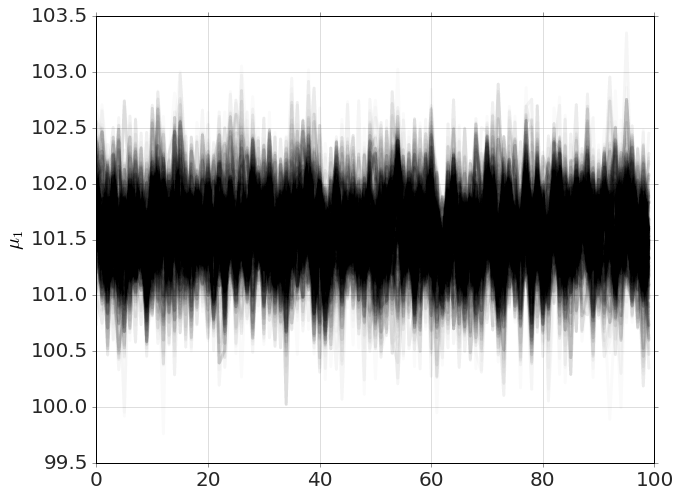
\includegraphics{SIE_MCMC_Best_Test/output_4_0.png}
\caption{Chains for parameter $mu_{1}$, the mean of the {\tt drug} group.}
\end{figure}

\begin{Shaded}
\begin{Highlighting}[]
\NormalTok{model.plot_distribution(}\StringTok{'mu1'}\NormalTok{)}
\end{Highlighting}
\end{Shaded}

\begin{figure}[htbp]
\centering
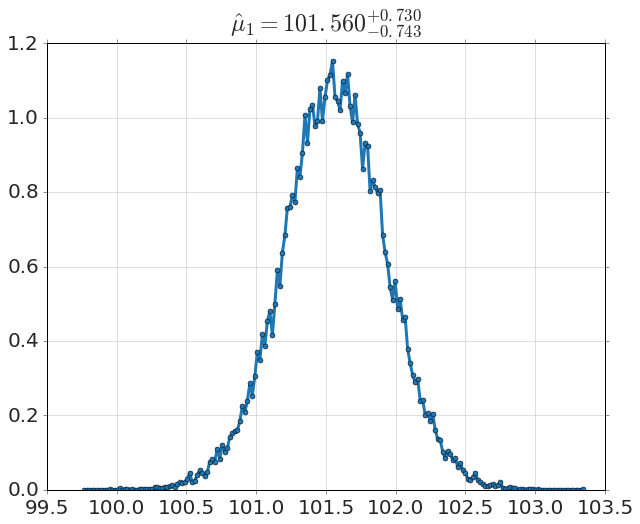
\includegraphics{SIE_MCMC_Best_Test/output_5_0.png}
\caption{Distribution for parameter $mu_{1}$, the mean of the {\tt drug} group.}
\end{figure}

\begin{Shaded}
\begin{Highlighting}[]
\NormalTok{model.plot_distribution(}\StringTok{'mu2'}\NormalTok{)}
\end{Highlighting}
\end{Shaded}

\begin{figure}[htbp]
\centering
\caption{Distribution for parameter $mu_{2}$, the mean of the {\tt placebo} group.}
\caption{png}
\end{figure}

\begin{Shaded}
\begin{Highlighting}[]
\NormalTok{model.plot_distribution(}\StringTok{r'$\textbackslash{}delta$=mu1-mu2'}\NormalTok{)}
\end{Highlighting}
\end{Shaded}

\begin{figure}[htbp]
\centering
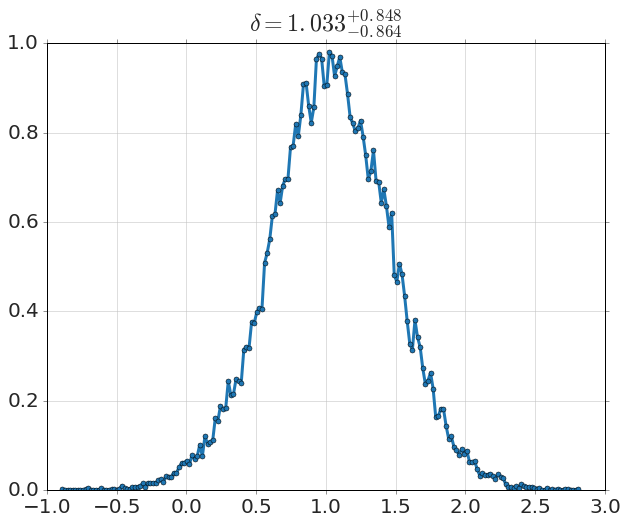
\includegraphics{SIE_MCMC_Best_Test/output_7_0.png}
\caption{Distribution for parameter $\delta$, the mean of the {\em difference} between the {\tt drug} group and the {\tt placebo} group.}
\end{figure}

We can clearly see from the distribution of $\delta$, as well as the credible ranges, that there is significant evidence for a non-zero effect.  We would want to extend this to include the effect size, and explore the prior probability of the the drug working, in order to reasonably assess whether this is an effect worth pursuing.  
